% diags.Rnw --
%
% Author: laurence kell <lauriekell@gmail.com>

%\VignetteIndexEntry{cpue}
%\VignetteIndexEntry{An R Package for read/wrting CPUE files and plotting data from a variety of fish stock assessment programs}
%\VignetteKeyword{CPUE, diagnostics, IO, read, write}


\documentclass[shortnames,nojss,article]{jss}

\usepackage[onehalfspacing]{setspace}
\usepackage{natbib} \bibliographystyle{plain}
\usepackage{graphicx, psfrag, Sweave}
\usepackage{enumerate}

\usepackage{booktabs,flafter} %,thumbpdf}
\usepackage{hyperref}

%\newcommand{\code}[1]{\texttt{#1}}
%\newcommand{\proglang}[1]{\textsf{#1}}
%\newcommand{\pkg}[1]{{\fontseries{b}\selectfont #1}}

\author{Laurence Kell\\ICCAT}
\Plainauthor{Laurence Kell}

\title{\pkg{diags}: \proglang{R} Tools for Catch per Unit Effort Analysis}
\Plaintitle{diags: R Tools for Catch per Unit Effort Analysis}

\Abstract{The \pkg{diags} package provides methods for plotting and summarising Catch per Unit Effort (CPUE) data used in fitting fish stock assessment methods. Programs for stock assessment are generally implemented as  standalone executable programs with their own text files for input and output files. \pkg{diags} provides a set of methods for reading these data and the results from fitting them nto R.}

\Keywords{\proglang{R}, CPUE, diagnsotics, residuals, stock assessment}
\Plainkeywords{R, CPUE, diagnsotics, residuals,  stock assessment}

\Address{
  Laurence Kell \\
  ICCAT Secretariat\\ 
  C/Coraz\'{o}n de Mar\'{\i}a, 8. \\
  28002 Madrid\\
  Spain\\ 
  
  E-mail: \email{Laurie.Kell@iccat.int}
}

%% need no \usepackage{Sweave.sty}




\begin{document}
\Sconcordance{concordance:diags.tex:diags.Rnw:%
1 58 1 1 29 34 1 1 4 17 1 1 4 6 1 1 2 4 0 1 2 12 1 1 2 1 0 1 1 4 0 1 2 %
3 1 2 2 23 1 1 2 1 0 1 2 1 1 12 0 1 2 17 1 1 2 1 0 1 1 3 0 1 2 3 1 1 2 %
1 0 1 1 3 0 1 2 8 1 1 2 1 0 1 1 3 0 1 2 2 1 1 2 4 0 1 2 4 1 1 2 1 0 6 1 %
3 0 1 2 24 1 1 7 10 0 1 2 7 1 1 2 1 0 2 1 1 2 2 1 1 5 8 0 1 2 9 1 1 2 1 %
0 2 1 1 3 9 0 1 2 9 1 1 6 9 0 1 2 6 1 1 6 9 0 1 2 10 1 1 2 1 0 1 8 10 0 %
1 2 6 1 1 2 1 0 1 7 9 0 1 2 6 1 1 9 12 0 1 2 6 1 1 7 10 0 1 2 5 1 1 7 %
10 0 1 2 22 1 1 4 1 2 19 1}


\tableofcontents
\newpage 

\section{introduction}

The \pkg{diags} package provides methods for plotting and summarising Catch per Unit Effort (CPUE) data used in fitting fish stock assessment methods. Programs for stock assessment are generally implemented as  standalone executable programs with their own text files for input and output files. \pkg{diags} provides a set of methods for reading these data and the results from fitting them nto R.

The stock assessment package for which there are R methods for reading text files are

\begin{itemize}
 \item \href{http://iccat.int/en/AssessCatalog.htm}{ASPIC} a biomass dynamic model fitted by maximising the likelihood 
 \item \href{http://iccat.int/en/AssessCatalog.htm}{BSP}  a Bayesian biomass dynamic model fitted using the SIR algorithm
 \item \href{http://www.ices.dk/committe/acom/wg/asoft/VPA/}{VPA Suite} Imput file format mainly used by ICES for virtual population analysis
 \item \href{http://iccat.int/en/AssessCatalog.htm}{VPA2Box} An age structured model based on virtual population analysis
 \item \href{http://www.multifan-cl.org}{Multifan-CL} A statistical, length-based, age-structured model
 \item \href{http://nft.nefsc.noaa.gov/Stock_Synthesis_3.htm}{Stock Synthesis} age and size structure assessment model
\end{itemize}


\section{Data}

The \code{readCpue} method reads data from the various stock assessment files into a commom data frame.
There is an example data frame in the package

\begin{Schunk}
\begin{Sinput}
> library(diags)
> data(rsdl)
> head(rsdl)
\end{Sinput}
\begin{Soutput}
   year        name  obs  hat residual residualLag   qqx   qqy qqHat
12 1967 Japan LL II 0.25 0.19     0.26        0.28  0.69  0.26  0.27
13 1968 Japan LL II 0.26 0.19     0.28        0.38  0.77  0.28  0.29
14 1969 Japan LL II 0.27 0.19     0.38        0.12  1.57  0.38  0.57
15 1970 Japan LL II 0.21 0.18     0.12        0.13  0.24  0.12  0.11
16 1971 Japan LL II 0.21 0.18     0.13       -0.20  0.36  0.13  0.15
17 1972 Japan LL II 0.14 0.18    -0.20       -0.30 -0.62 -0.20 -0.19
\end{Soutput}
\end{Schunk}

The columns identify the observations (\code{year,name} and may include other covariates such as age, season, etc.), the original observations (\code{obs}) and the fitted values and the residuals (\code{obs,hat}) if \code{diags} has been used to read in the data, the residuals with a lag
of 1 (\code{residualLag}) and the quanitiles (\code{qqx,qqy,qqHat}) assumming a normal distribution.

In some assessment packages the data are in a specific file in other cases the data are in a suite of files found in a dir. Therefore the \code{readCpue} takes either a file or a dir as irs first arguemnt depending on the assessment method e.g. reading in from vpa2box and SS


\begin{table}\caption{plot}\begin{tabular}{|l|p{12cm}|} 
\hline\multicolumn{2}{|c|}{Syntax} \\
\hline 
x       & \code{vector} values of one variable of interest \\ 
data   	& \code{data.frame} other variables\\ 
geom		& \code{ggplot object} that sets the type of plot to construct, i.e. \code{point, line, histogram}. \\ 
\hline 
\end{tabular}\end{table}
Creating a scatter plot is therefore very similar to how it is done using base R, i.e.


\begin{Schunk}
\begin{Sinput}
> u2box=readCpue("unisex09.c01","2box")
> uSS  =readCpue("myDir","ss")
\end{Sinput}
\end{Schunk}

\code{readCpue} only reads in the data as input to a stock assessment, \code{diags} reads the residuals and and covariates as well.


\begin{Schunk}
\begin{Sinput}
> u2box=readCpue("unisex09.c01","2box")
> uSS  =readCpue("myDir","ss")
\end{Sinput}
\end{Schunk}

There is also the \code{writeCpue} method  for writing the various input files

\section{Transformations}

For plotting and analysis the data may need to be transformed, e.g. observations scaled so that
they can be compared, or pearson residuals computed. This can be done as required using \code{transform}
and \code{plyr}, e.g. to standardise the residuals or scale them so that they lie between 0 and 1.

\begin{Schunk}
\begin{Sinput}
> stdz(  rnorm(10,1,.3))
> minMax(rnorm(10,1,.3))
\end{Sinput}
\end{Schunk}

If you wish to scale the residuals within a series then the \pkg{plyr} can be used which implements the split-apply-combine strategy for \pkg{R} e.g.

\begin{Schunk}
\begin{Sinput}
> rsdl=ddply(rsdl, .(name), transform, stdRsdl=stdz(residual))
\end{Sinput}
\end{Schunk}

One common definition, known as the Pearson residual, is as follows, however the definition depends on the law of large numbers, so it works less well where the number of points in each series is relatively small. Therefore in this anaysis we used the raw residuals, but the residuals could be transformed as required.
 
There may be other analyses that are useful to run on the raw data, e.g. running a GAM to calculate a common trend that the individual series can be compared to. I.e. to look for trends that may be different from the others. This can be done by fitting a smoother to year and a series effect, the latter scales the series so that they can be compared, e.g.

\begin{Schunk}
\begin{Sinput}
> library(gam)
> gm  =gam(log(obs)~lo(year)+name,data=rsdl)
> rsdl=data.frame(rsdl,gam=predict(gm),gamRsdl=residuals(gm))
> scl =coefficients(gm)[3:9]
> names(scl)=substr(names(scl),5,nchar(names(scl)))
> rsdl=transform(rsdl,scl=scl[as.character(name)])
> rsdl[is.na(rsdl$scl),"scl"]=0
\end{Sinput}
\end{Schunk}

\section{Plotting}

Plotting is done using \hyperref[http://had.co.nz/ggplot2/]{ggplot2}, a plotting package based on the grammar of graphics. For those already familar with lattice a comparison can be found at \hyperref[http://had.co.nz/ggplot/vs-lattice.html]{ggplot v lattice} and \hyperref[http://learnr.wordpress.com/2009/06/28/ggplot2-version-of-figures-in-lattice-multivariate-data-visualization-with-r-part-1/]{learning R}. Searching for ggplot2 in google images will throw up lots of examples with code and there is a very active \href{users mailing list}{}.

\subsection[gg]{Grammar of Graphics}

When producing a graphic you have to map data to the visual properties of geometric shapes (e.g. points, lines areas). This
may require statistical transformations of the data, a coordinate system that postions the geometric objects on the page
and facetting where mutiple plots can be generated. Each of these tasks are independent and the grammar breaks theses into four 
%components \emph{Geoms, Aesthetics, Coordinates and Facetting}. 

First we load up FLR and an example data set based on North Sea plaice. ggplot uses data in the form of a data.frame so we 
next have to convert the FLR object to a data.frame. 

Facetting creates individual panels by the facetting variables, while themes allow you to prettify the plots. 


\clearpage
\section{Exploratory Data Analysis}

First the CPUE time series are plotted using \code{geom_line} to plot the common trend as estimated by the GAM,
then \code{geom_smooth} fits a loess by series and then \code{geom_point} is used to overlay the original observations. \code{facet_wrap} then plots the series individually. \code{theme_ms} is a bespoke theme to change the look of the plot from the default.

\begin{figure}\begin{center}
\begin{Schunk}
\begin{Sinput}
> ggplot(rsdl)+ geom_line(aes(year,exp(gam)),col="red")  +
+               geom_smooth(aes(year,obs),se=FALSE)      +           
+               geom_point(aes(year,obs,col=name))       +
+               facet_wrap(~name,ncol=1,scale="free_y")  +
+               theme_ms(legend.position="none")         +
+               xlab("Year") + ylab("Index")
\end{Sinput}
\end{Schunk}
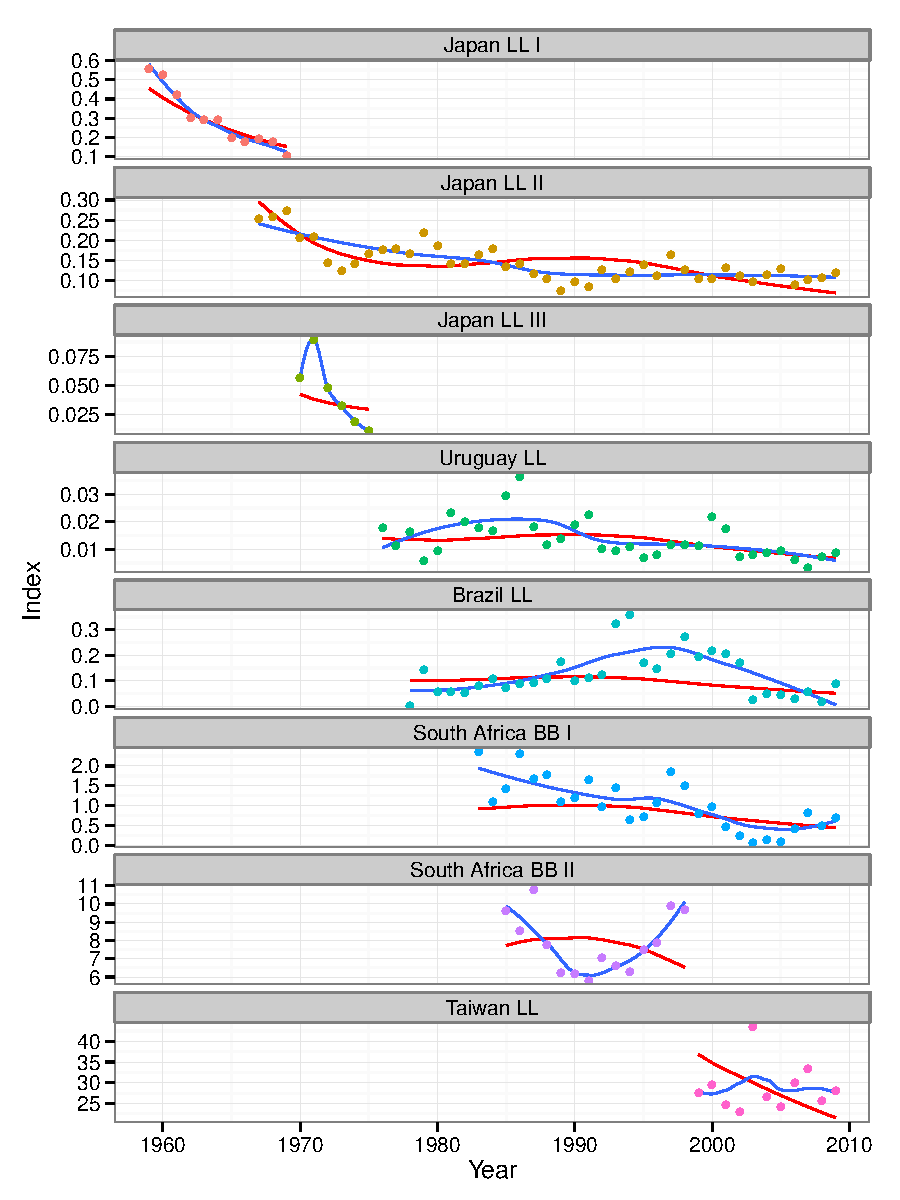
\includegraphics{diags-008}
\caption{\bf{Plot of indices of abundance, points are the observed index values and the blue a 
lowes fit to the points by index. The red line is GAM fitted to lo(year) and fleet.}}
\label{cpue:1} 
\end{center}\end{figure}

The correlations between indices can be seen by plotting the indices against each other 

\begin{figure}\begin{center}
\begin{Schunk}
\begin{Sinput}
> uMat=ddply(rsdl,.(name),transform, obs=stdz(obs))
> uMat=cast(uMat,year~name,value="obs")
> uMat=uMat[apply(uMat,1,function(x) !all(is.na(x))),]
> pM=plotmatrix(uMat[,-c(1:2,4)])
> pM$layers[[2]]=NULL
> mns=ddply(subset(pM$data,!(is.na(x) & !is.na(y))),.(xvar,yvar), function(x) mean(x$y,na.rm=T))
> pM+geom_hline(aes(yintercept=V1),data=mns,col="red") +
+    geom_smooth(method="lm",fill="blue", alpha=0.1)  + 
+    theme(legend.position="bottom")                   +
+    xlab("Index")+ylab("Index")                       +
+    theme_ms()
\end{Sinput}
\end{Schunk}
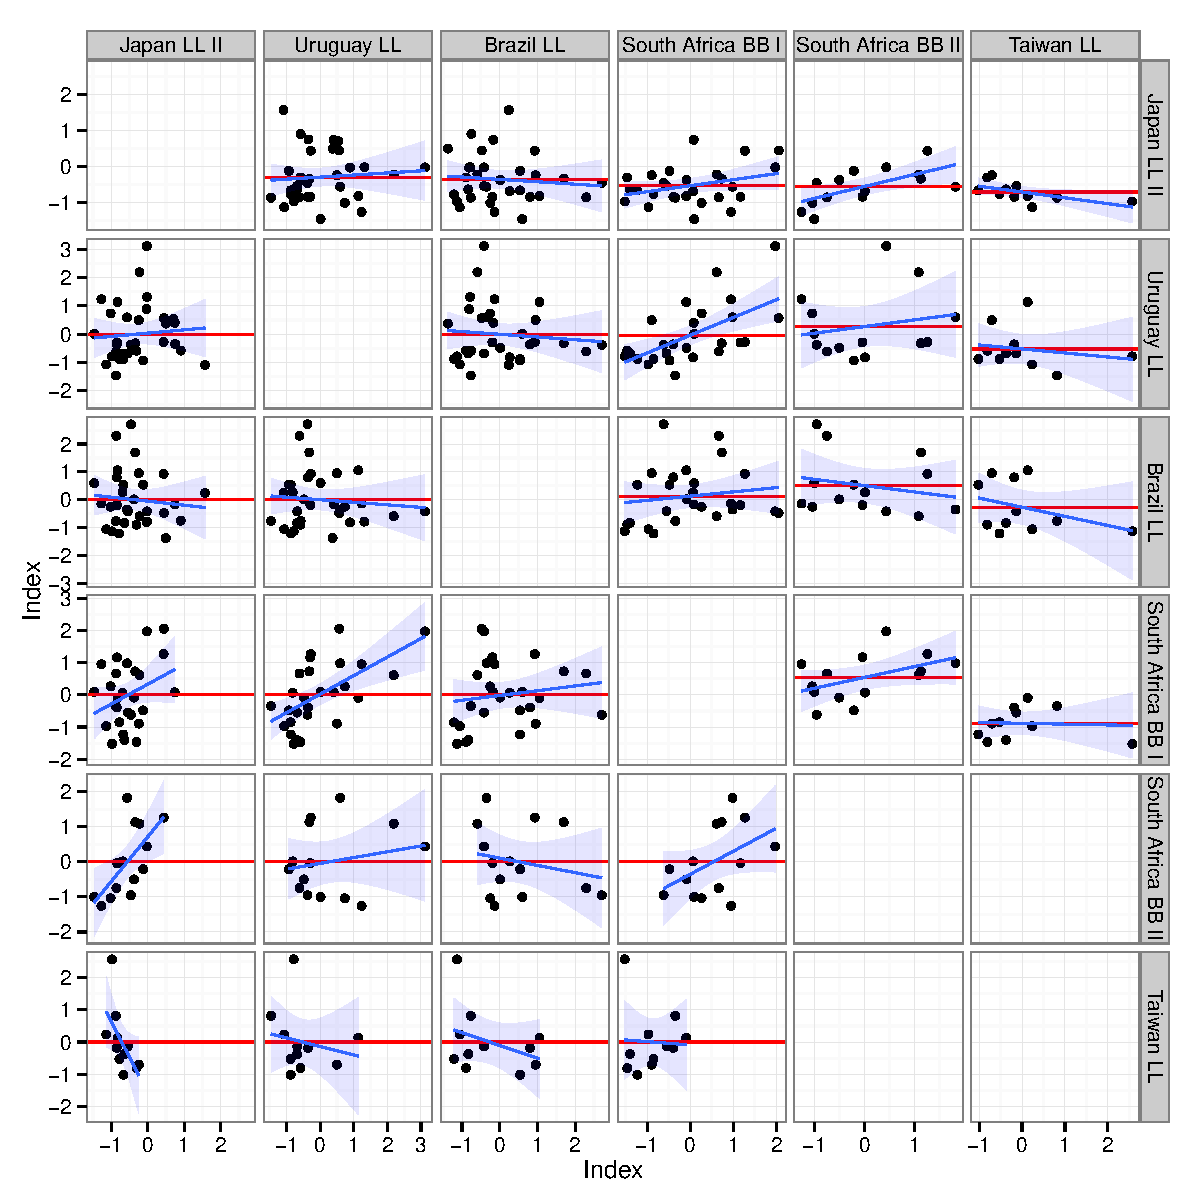
\includegraphics{diags-009}
\caption{\bf{Pairwise scatter plots of the indices of abundance, blue lines are linear regressions 
fitted to the points, the shade area is the standard error of predicted means and the red line is 
the mean of the points on the y-axis.}}
\label{cpue:2}
\end{center}
\end{figure}

The indices are then be grouped based on a cluster analysis

\begin{figure}\begin{center}
\begin{Schunk}
\begin{Sinput}
> cr=cor(uMat[,-1],use="pairwise.complete.obs")
> dimnames(cr)=list(gsub("_"," ",names(uMat)[-1]),gsub("_"," ",names(uMat)[-1]))
> cr[is.na(cr)]=0
> corrplot(cr,diag=F,order="hclust",addrect=2)  +          
+              theme(legend.position="bottom")  +
+              theme_ms()
\end{Sinput}
\begin{Soutput}
NULL
\end{Soutput}
\end{Schunk}
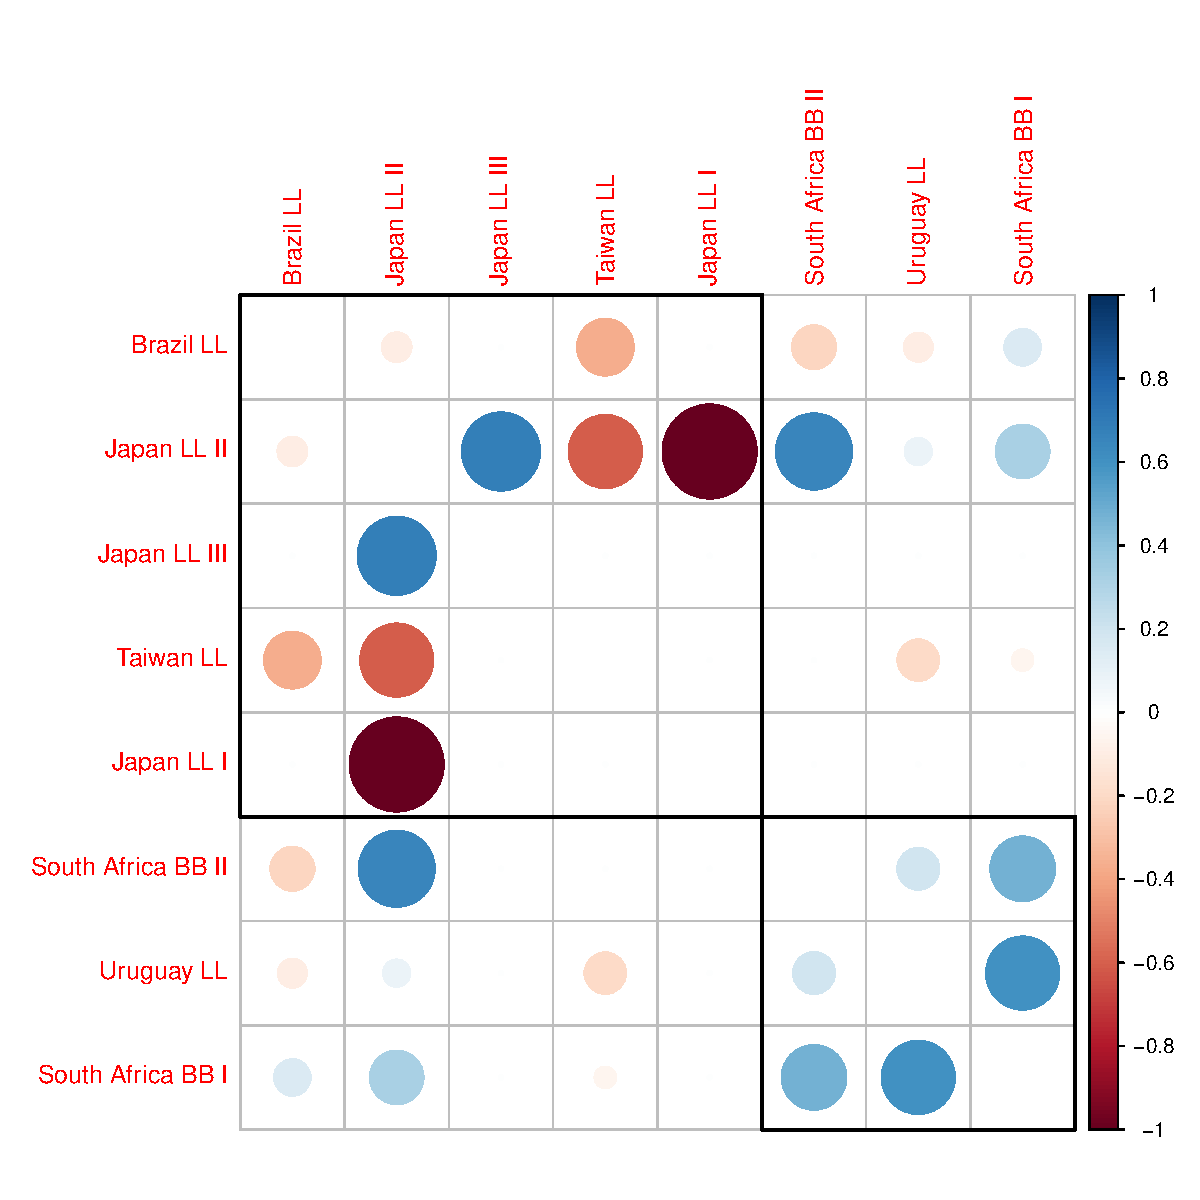
\includegraphics{diags-010}
\caption{\bf{A plot of the correlation matrix for the indices, blue indicate a positive correlation 
and red negative. the order of the indices and the rectanglur boxes are chosen based on a hierarchical 
cluster analysis using a set of dissimilarities for the indices being clustered.}}
\label{cpue:3}
\end{center}
\end{figure}

To explore the groupings further series within a cluster are plotted together

\begin{figure}\begin{center}
\begin{Schunk}
\begin{Sinput}
> ggplot(subset(rsdl,name %in% c("Japan LL II","Japan LL III","South Africa BB II")))+
+              geom_point(aes(year,exp((gam+gamRsdl)-scl),col=name))+
+              geom_smooth(aes(year,exp(gam+gamRsdl-scl),group=name,col=name),se=T,fill="blue", alpha=0.1)+
+              theme_ms(legend.position="bottom") +
+              xlab("Year") +ylab("Index")
\end{Sinput}
\end{Schunk}
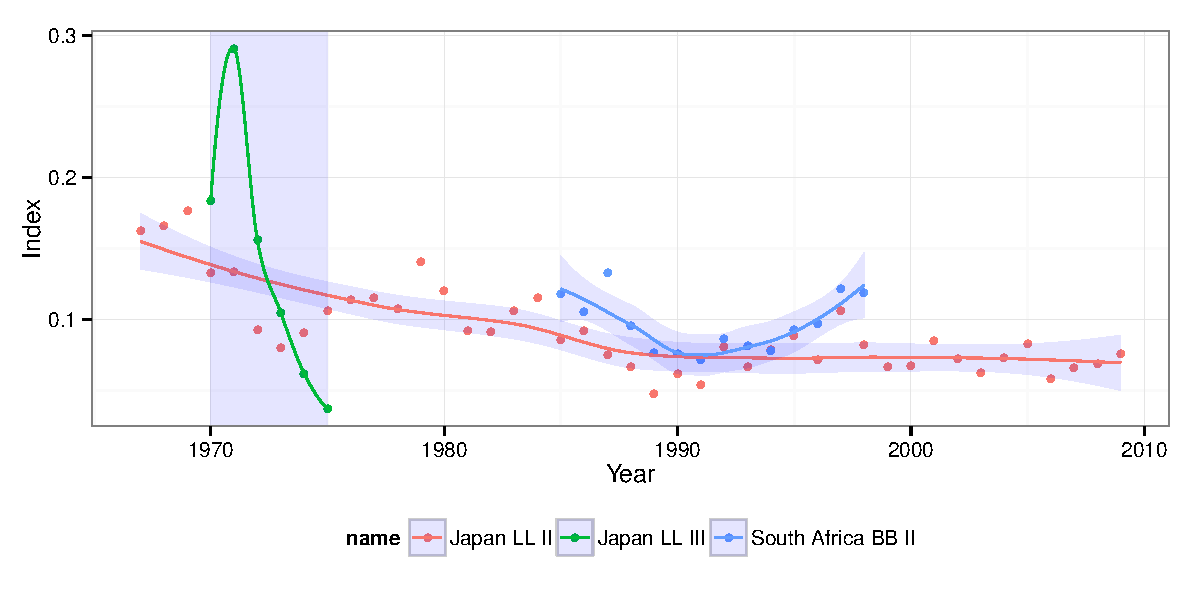
\includegraphics{diags-011}
\caption{\bf{Plots of Japan LL II, Japan LL III and South Africa BB II indices, lowess regressions and SEs are shown for each series.}}\caption{\bf{Plots of South Africa BB I, South Africa BB II and Uruguay LL indices, lowess regressions and SEs are shown for each series.}}
\label{cpue:4}
\end{center}
\end{figure}


\begin{figure}\begin{center}
\begin{Schunk}
\begin{Sinput}
>     ggplot(subset(rsdl,name %in% c("South Africa BB I","South Africa BB II","Uruguay LL"))) +   
+             geom_point(aes(year,exp((gam+gamRsdl)-scl),col=name))+
+              geom_smooth(aes(year,exp(gam+gamRsdl-scl),group=name,col=name),se=T,fill="blue", alpha=0.1)+
+              theme_ms(legend.position="bottom")  +
+              xlab("Year") +ylab("Index")
\end{Sinput}
\end{Schunk}
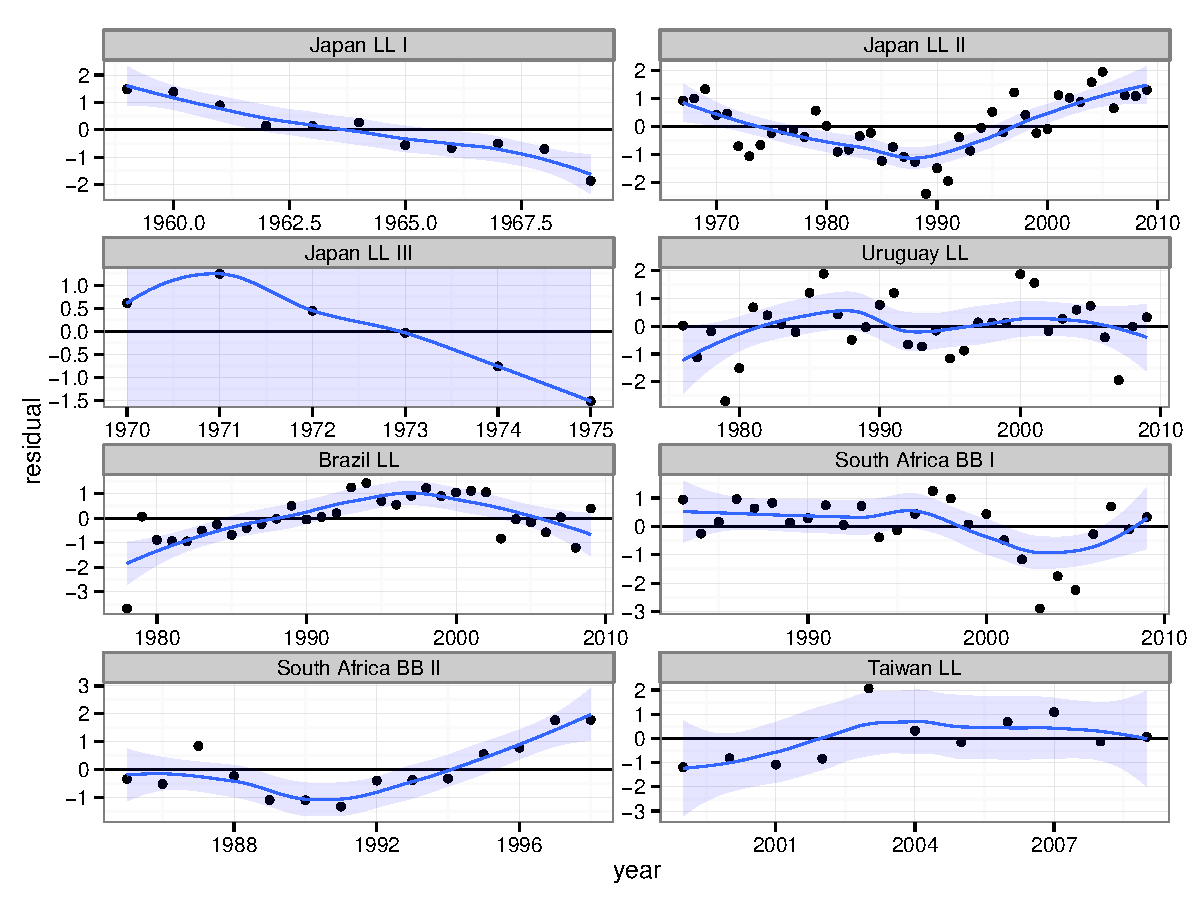
\includegraphics{diags-012}
\caption{\bf{Observed CPUE verses fitted, blue line is a linear resgression fitted to points, black the y=x line.}}
\label{cpue:5}
\end{center}
\end{figure}

\clearpage
\section{Residual Analysis}

Next the fit to the indices is evaluated by plotting the residuals. The first plot is of the observed and the predicted values. Since $U=qB$, i.e. the index is assumed to be proportional to stock size the points should fall either side of the $y=x$ line.    

\begin{figure}\begin{center}
\begin{Schunk}
\begin{Sinput}
> dat=ddply(rsdl, .(name), with, data.frame(obs=stdz(obs),hat=stdz(hat)))
> ggplot(dat) +
+           geom_abline(aes(0,1))                         +
+           geom_point( aes(obs,hat))                     +
+           stat_smooth(aes(obs,hat),method="lm",fill="blue", alpha=0.1)       +
+           facet_wrap(~name,ncol=3)                      +
+           theme_ms(legend.position="bottom")            +
+           xlab("Fitted") + ylab("Observed")
\end{Sinput}
\end{Schunk}
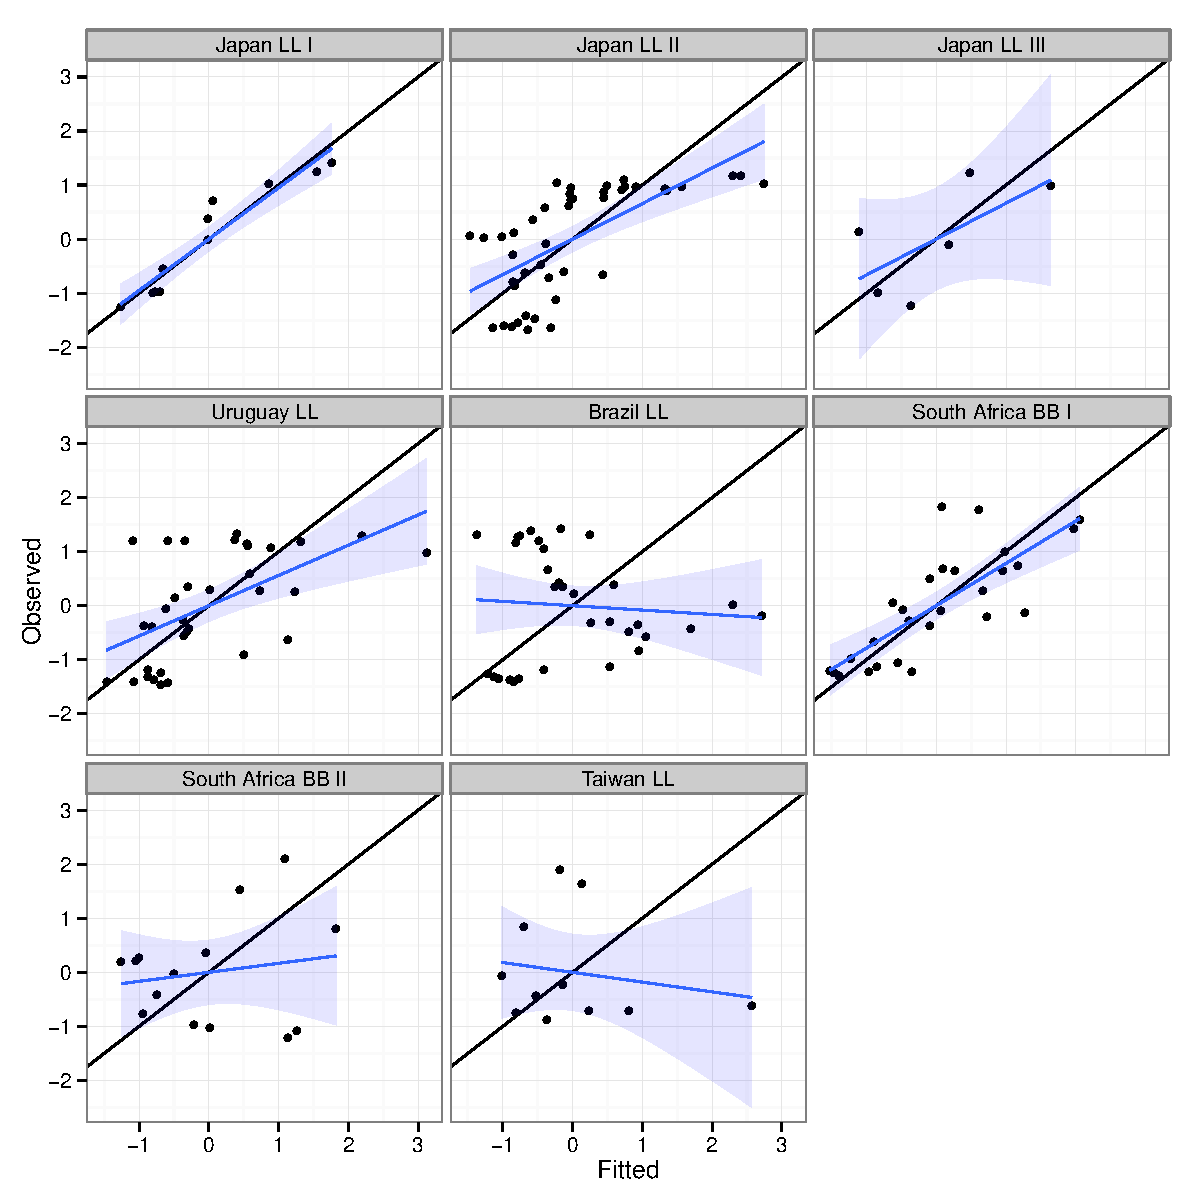
\includegraphics{diags-013}
\caption{\bf{Observed CPUE verses fitted, blue line is a linear resgression fitted to points, black the y=x line.}}
\label{residual:1}
\end{center}
\end{figure}

Departures from the assumption that the index is proportional to the stock can also be seen by plotting the residuals by time. 
\begin{figure}\begin{center}
\begin{Schunk}
\begin{Sinput}
> dat=ddply(rsdl, .(name), transform, residual=stdz(residual,na.rm=T))
> ggplot(aes(year,residual),data=dat) +
+   geom_hline(aes(yintercept=0))      +
+   geom_point()                       +
+   stat_smooth(,method="loess",se=T,fill="blue", alpha=0.1)  +
+   facet_wrap(~name,scale="free",ncol=2)   +
+              theme_ms() 
\end{Sinput}
\end{Schunk}
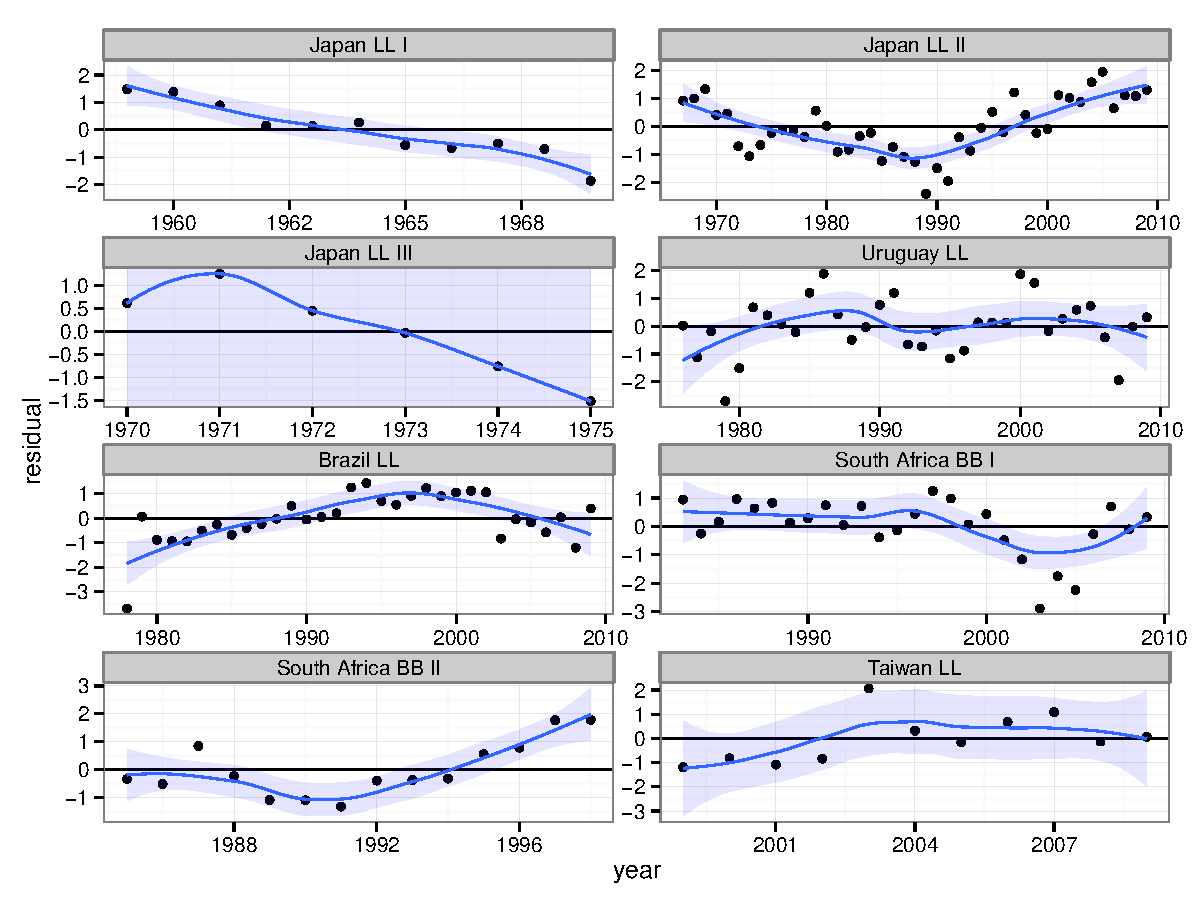
\includegraphics{diags-014}
\caption{\bf{Residuals by year, with lowess smoother and SEs.}}
\label{residual:2}
\end{center}
\end{figure}

Autocorrelated residuals may mean that the estimated parameters are biased, autocorrelation can be checked by plotting the residuals against each other with a lag e.g.
\begin{figure}\begin{center}
\begin{Schunk}
\begin{Sinput}
> ggplot(rsdl)                                              +
+   geom_point( aes(residual,residualLag))                  +
+   stat_smooth(aes(residual,residualLag),method="lm",se=T,fill="blue", alpha=0.1)      +
+   geom_hline(aes(yintercept=0))                           +
+   facet_wrap(~name,scale="free",ncol=3)                   +
+   xlab(expression(Residual[t])) + 
+   ylab(expression(Residual[t+1])) +
+   theme_ms(legend.position="bottom")  
\end{Sinput}
\end{Schunk}
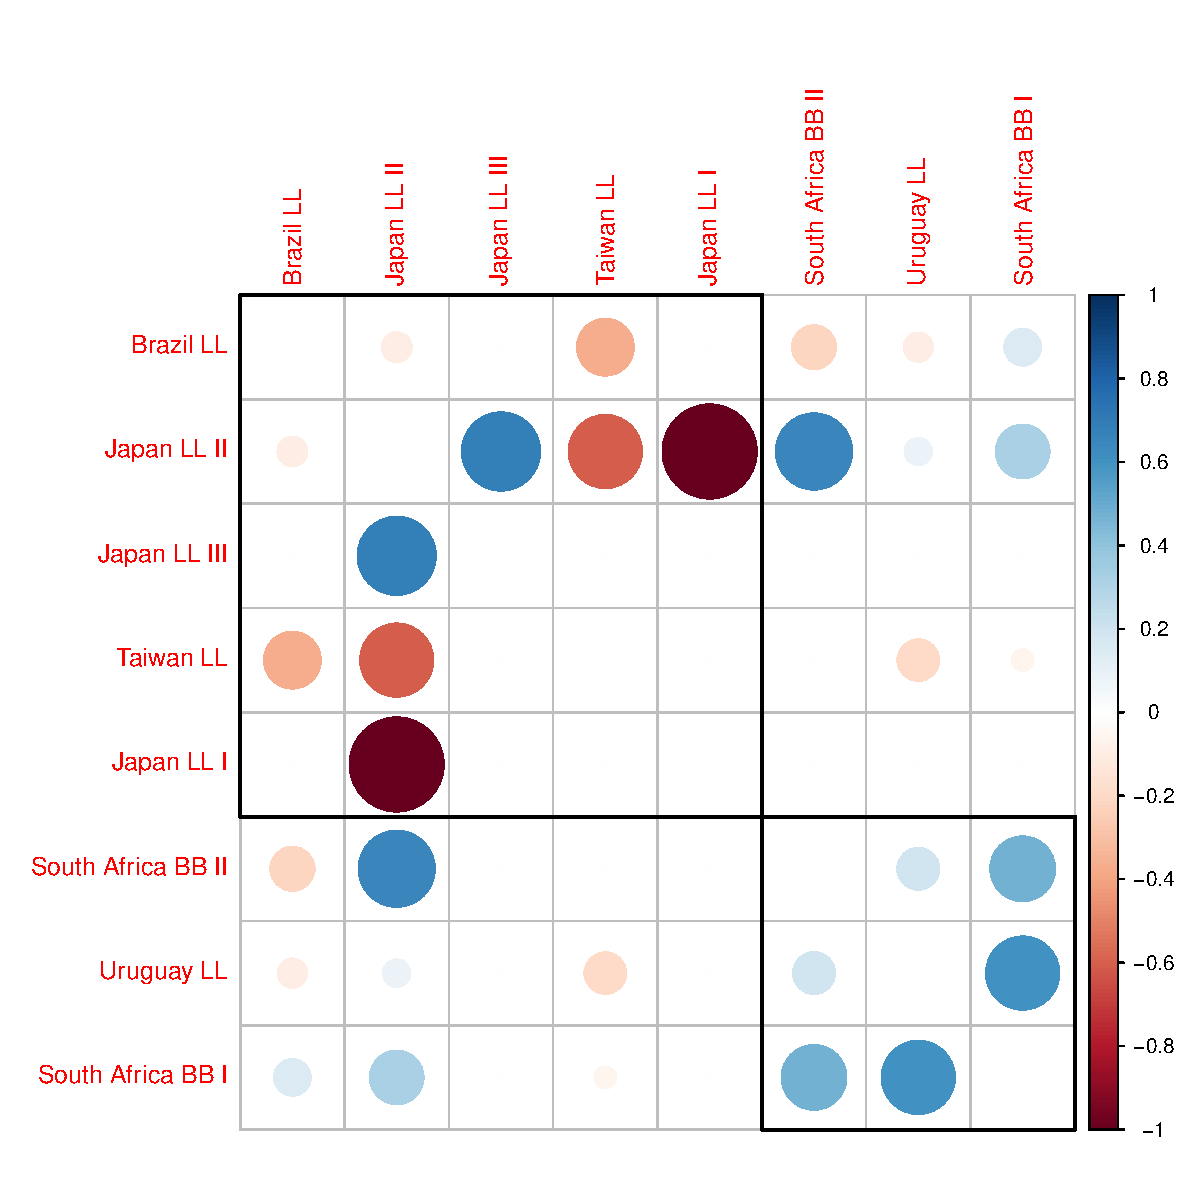
\includegraphics{diags-015}
\caption{\bf{Plot of autocorrelation, i.e. $residual_{t+1}$ verses $residual_{t}$.}}
\label{residual:3}
\end{center}
\end{figure}

The error dostribution can be checked by plotting the observed and the predicted quantiles for a given distribution e.g. for the normal distributuion
\begin{figure}\begin{center}
\begin{Schunk}
\begin{Sinput}
> ggplot(rsdl)                                           +
+   geom_point( aes(qqx,qqy))                            +
+   stat_smooth(aes(qqx,qqHat),method="lm",se=T,fill="blue", alpha=0.1)         +
+   facet_wrap(~name)                                    +
+   theme_ms(legend.position="bottom")                   +
+              theme_ms()
\end{Sinput}
\end{Schunk}
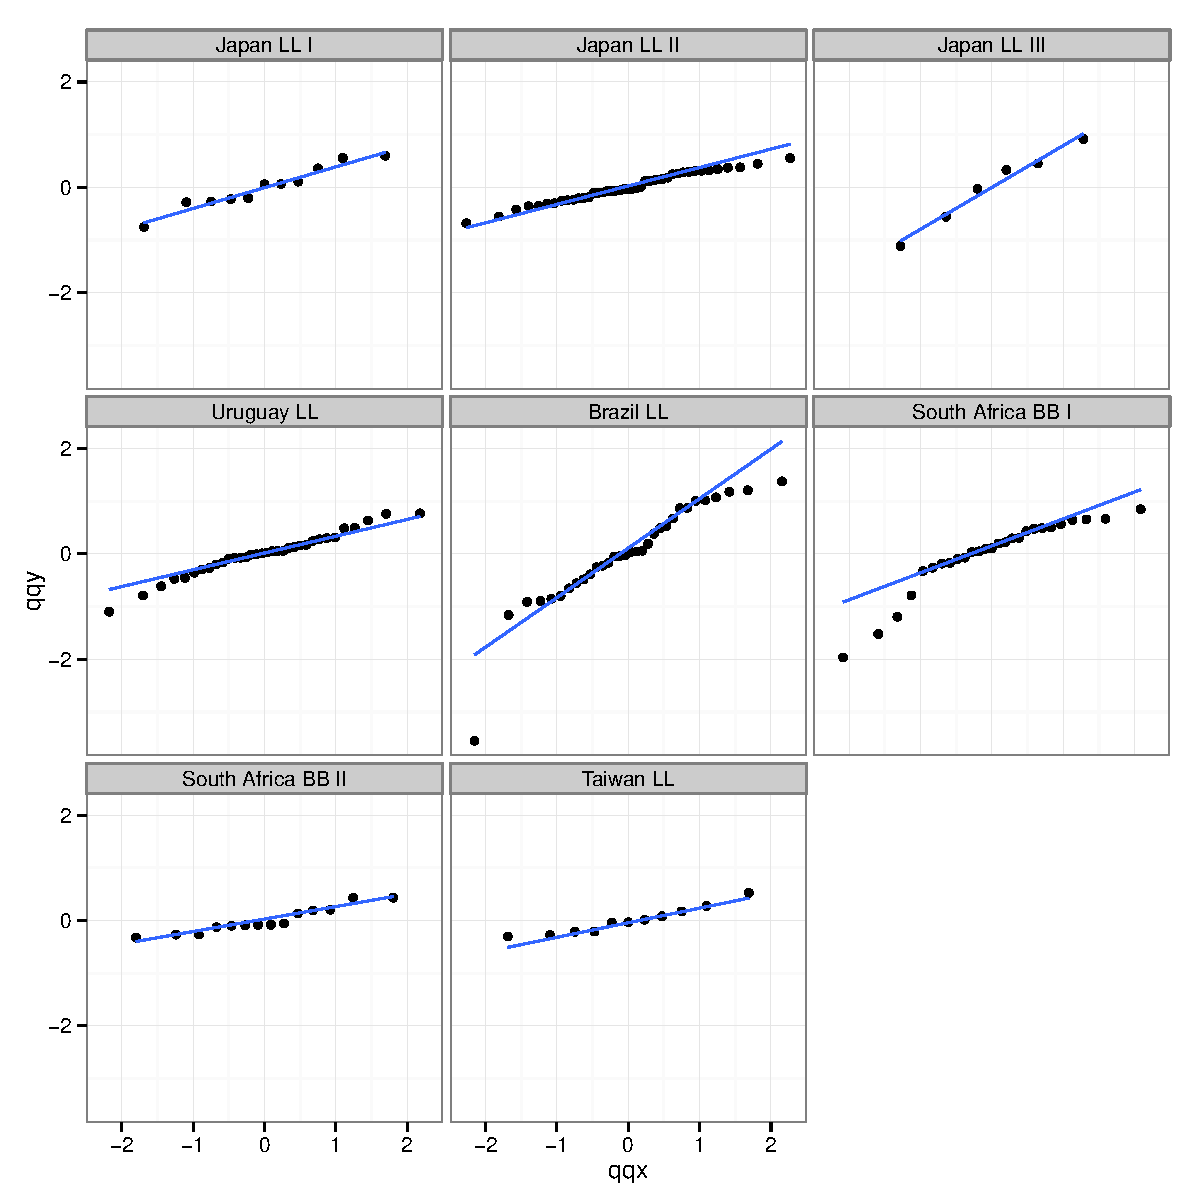
\includegraphics{diags-016}
\caption{\bf{Quantile-quantile plot to compare residual distribution with the normal distribution.}}
\label{residual:4}
\end{center}\end{figure}

The variance 
\begin{figure}\begin{center}
\begin{Schunk}
\begin{Sinput}
> ggplot(aes(hat, residual),data=rsdl)   +
+   geom_hline(aes(yintercept=0))         +
+   geom_point()                          +
+   stat_smooth(method="loess",span=.9,fill="blue", alpha=0.1)   +
+   facet_wrap(~name,scale="free",ncol=3) +
+              theme_ms()
\end{Sinput}
\end{Schunk}
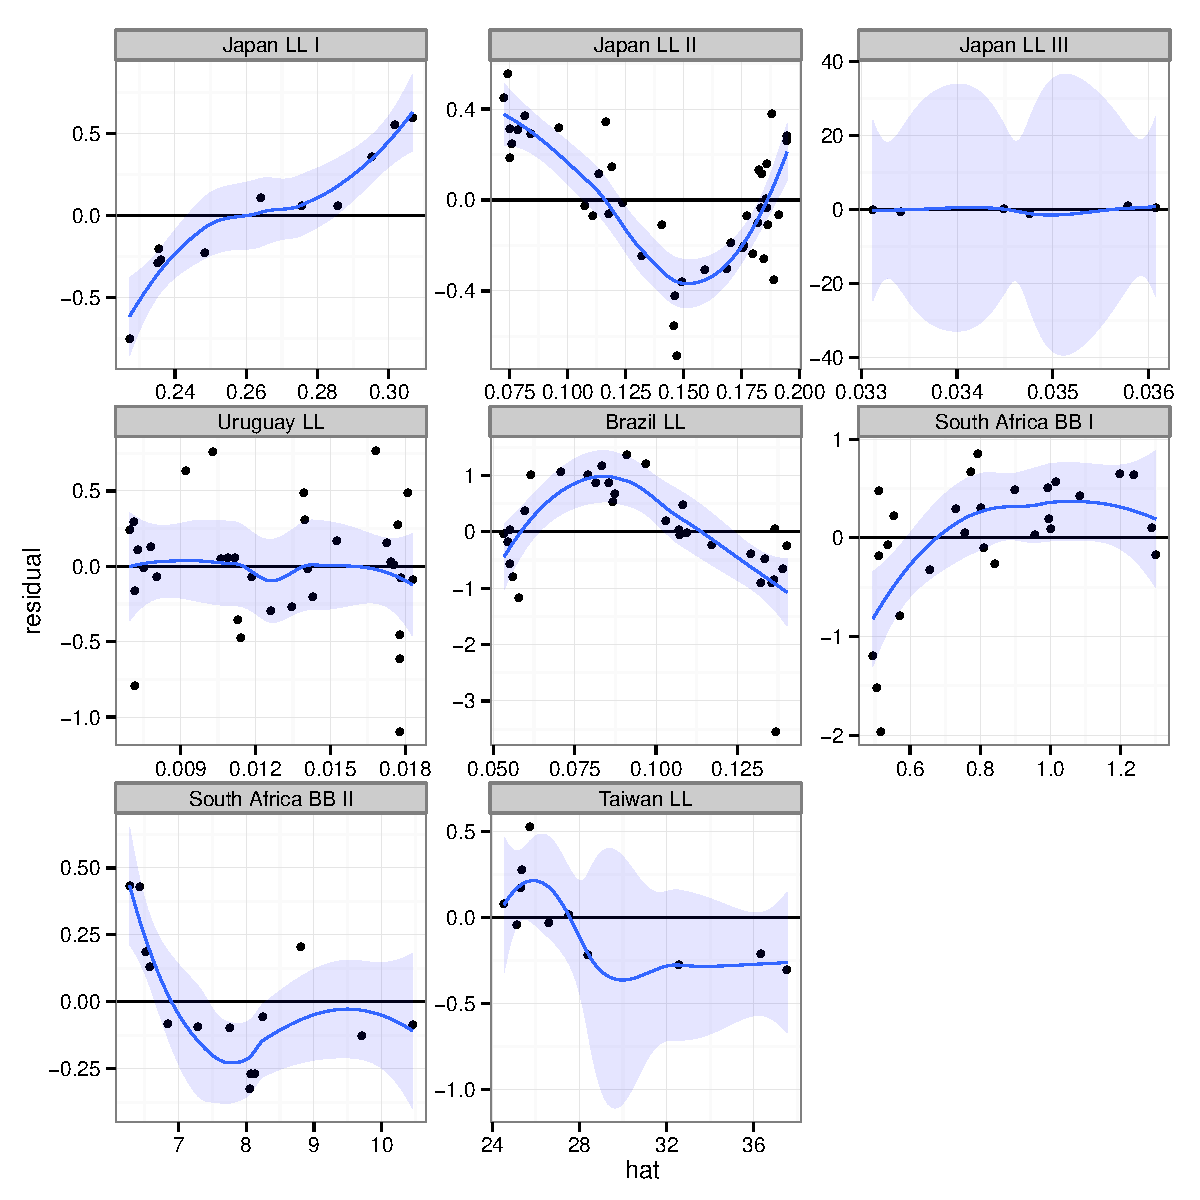
\includegraphics{diags-017}
\caption{\bf{Plot of residuals against fitted value, to check variance relationship.}}
\label{residual:5}
\end{center}\end{figure}

\clearpage
\section{Standardised CPUE}

Most CPUE series used in stock assessment have been standardised using a Generalised Linear Model (GLM). This
requires choosing an appropriate error distribution, variance function andlink function \cite{mccullagh1989generalized}.

The best way to check these assumptions are by plotting, best
performed for a model that included all the main factors (i.e the most-complex model) since if the most
complex model isnt a reasonable fit, then any simpler models that are selected will fit adequately because if they
didn't they wouldn't be selected. 

Going clockwise from the top left in figure~\ref{glm} the first panel is a q-q plot to check that the residuals
follow a normal distribution, the standardised deviance residuals are then plotted against the fitted values to check for
systematic departures from the assumptions underlying the error distribution, then thethe absolute values of the
residuals against the fitted values as a check of the assumed variance function and finally the dependent variable
against the linear predictor function as a check of the assumed link function \cite{ortiz2004alternative}.


\begin{figure}\begin{center}
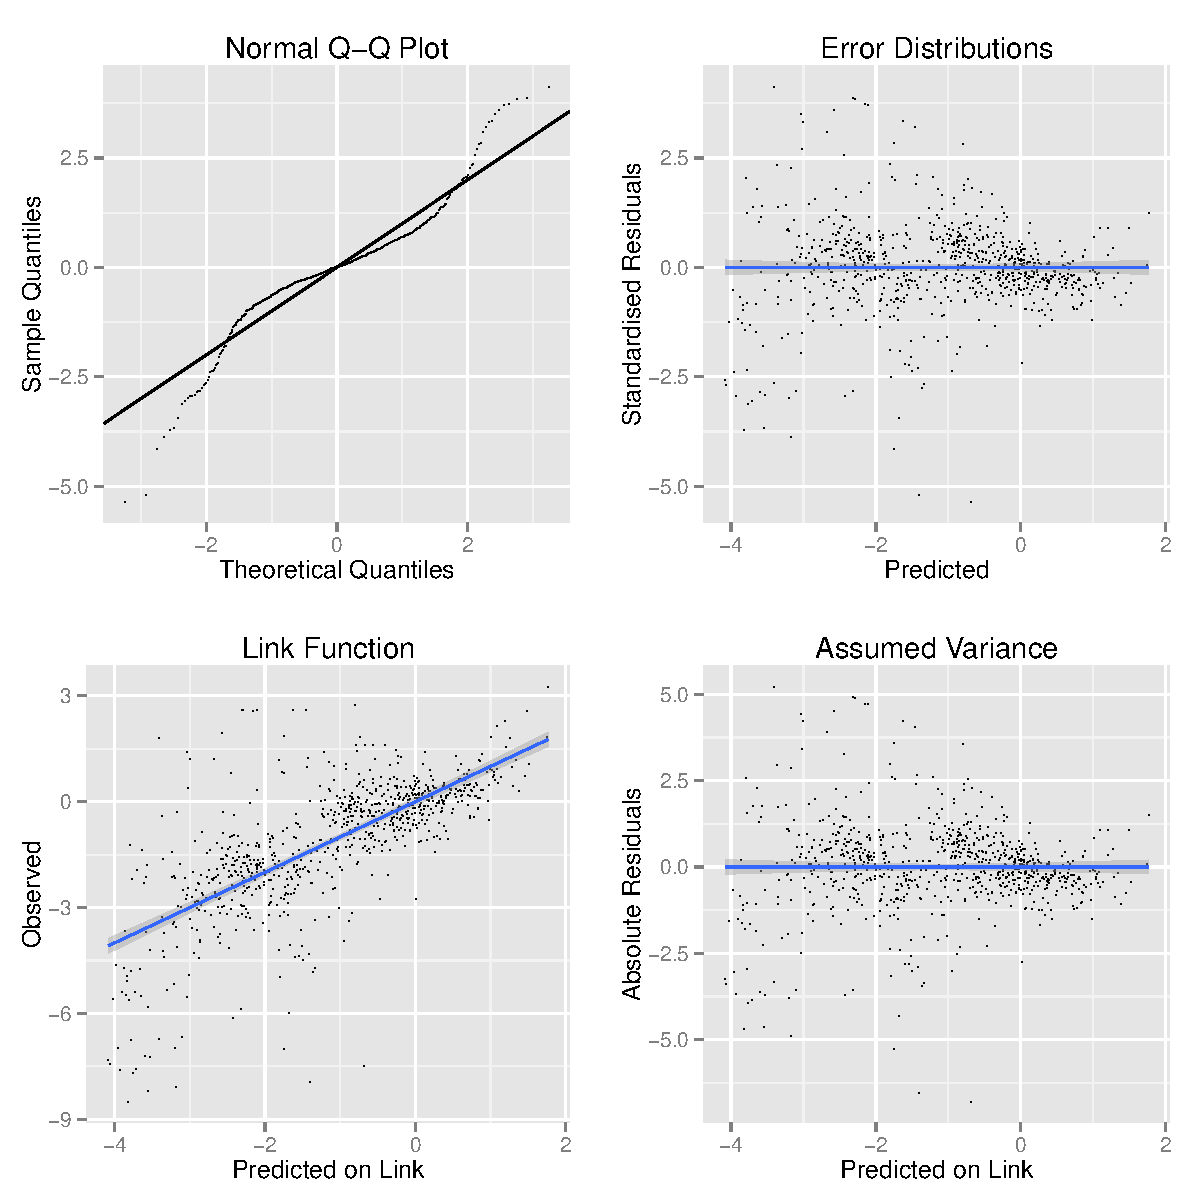
\includegraphics{diags-018}
\caption{\bf{Plot of residuals against fitted value, to check variance relationship.}}
\label{glm}
\end{center}\end{figure}




\newpage
\bibliography{refs} 
\bibliographystyle{abbrvnat}

\end{document}

\clearpage
\section{Hessian}

\clearpage
\section{MCMC}

\clearpage
\section{Simulation}

